\documentclass[10pt,letterpaper]{article}

\usepackage{psepress}
\usepackage{enumitem}
\usepackage{pgfplots}
\pgfplotsset{compat=1.18}

\renewcommand{\pseactivatearticlebodygeometry}{}
\captionsetup{font=footnotesize}
\newcolumntype{L}[1]{>{\RaggedRight\arraybackslash}p{#1}}
\DeclareRobustCommand{\artifact}[1]{%
  {\begingroup\urlstyle{tt}\footnotesize\nolinkurl{#1}\endgroup}%
}
\DeclareRobustCommand{\codeid}[1]{%
  {\begingroup\urlstyle{tt}\nolinkurl{#1}\endgroup}%
}
\setlist{nosep,leftmargin=*}
\emergencystretch=3em

\renewcommand{\PaperTitle}{Supplementary Material: Gate-Based Quantum Optimization for Discrete Process Design: A Repair-Aware Benchmark}
\renewcommand{\PaperAuthors}{%
Yirang ~Park\textsuperscript{a}
and David E. ~Bernal Neira\textsuperscript{a}}
\renewcommand{\PaperAffiliations}{%
\textsuperscript{a} Davidson School of Chemical Engineering, Purdue University, West Lafayette, IN 47907, USA\\
}
\renewcommand{\PaperAbstract}{%
This supplement provides four sections of supporting material for the
main manuscript. Section~1 describes the computational environment and
data availability. Section~2 reports numerical validation checks supporting
the manuscript claims, including the surrogate rank audit. Section~3 derives
the exact auxiliary-repair decomposition that reduces per-sample repair to
34 comparisons. Section~4 documents algorithm parameters and hardware
execution metadata for the variational and IBM~Quantum pilot experiments.
}
\renewcommand{\PaperKeywords}{%
supplementary material, quantum optimization, process design, reproducibility}
\renewcommand{\HeaderArticleType}{Supplementary Material}
\renewcommand{\HeaderReviewType}{Peer Reviewed Conference Proceeding}
\renewcommand{\HeaderConference}{FOCAPO-CPC 2027}
\renewcommand{\HeaderLocation}{Tucson, Arizona, USA, 10-14 January 2027}
\renewcommand{\FooterJournalInfo}{Syst Control Trans V:XXXX-YYYY (2027), Supplement}
\renewcommand{\FirstPageFooterID}{[DOI\_DoNotChange]}
\renewcommand{\BodyPageFooterID}{[LAPSE\_DoNotChange]}

\begin{document}
\psemaketitle

\section{Computational Environment and Data Availability}
\label{sec:supp-repository}

All scripts, data files, and circuit records for this case study are archived at
\url{https://github.com/SECQUOIA/pse-quantum-discrete-optimization} under
\codeid{case-studies/ds-mfg-qubo-qiskitopt/}.
The repository environment can be verified with
\texttt{julia --project=. scripts/smoke\_test.jl}, which imports all packages,
checks required artifacts, and validates cached summary values against recorded
checksums.
Table~\ref{tab:supp-software-env} lists the pinned software versions used
to produce the results in the main manuscript.

\begin{table*}[t]
\centering
\footnotesize
\caption{Pinned software environment for the DS-MFG case study. Version
         specifications are recorded in
         \artifact{case-studies/ds-mfg-qubo-qiskitopt/Project.toml},
         \artifact{Manifest.toml}, and
         \artifact{CondaPkg.toml}.}
\label{tab:supp-software-env}
\setlength{\tabcolsep}{3pt}
\begin{tabular}{L{0.22\linewidth}L{0.45\linewidth}L{0.25\linewidth}}
\hline
Layer & Component and version & Configuration file \\
\hline
Julia optimization wrapper &
\texttt{QiskitOpt.jl} v0.7.0. &
\artifact{Project.toml}; \artifact{Manifest.toml}. \\
\hline
Julia QUBO stack &
\texttt{QUBODrivers.jl} v0.6.1, \texttt{QUBOTools.jl} v0.13.0,
\texttt{QUBO.jl} v0.6.0. &
\artifact{Project.toml}; \artifact{Manifest.toml}. \\
\hline
Python bridge &
Qiskit 2.3.1, Qiskit Aer 0.17.2, Qiskit Optimization 0.7.0,
Qiskit IBM Runtime 0.46.1, NumPy 2.2.6, SciPy 1.15.3. &
\artifact{CondaPkg.toml}. \\
\hline
Classical solver &
Gurobi 13.0.2 (\texttt{PoolSearchMode=2}, \texttt{PoolSolutions=36}). &
\artifact{scripts/run\_classical\_baselines.jl}. \\
\hline
\end{tabular}
\end{table*}

\clearpage

\section{Numerical Validation}
\label{sec:supp-validation}

\begin{table*}[t]
\centering
\footnotesize
\caption{Numerical validation checks supporting the manuscript claims.}
\label{tab:supp-validation-facts}
\setlength{\tabcolsep}{3pt}
\begin{tabular}{L{0.25\linewidth}L{0.40\linewidth}L{0.27\linewidth}}
\hline
Check & Value & Anchor \\
\hline
Exact repaired optimum &
$F(y^\star)=11.7095$ at flow
\codeid{1001110100111100011}; certified by exact enumeration over all
$2^{19}$ flow assignments. &
\artifact{ds\_mfg\_reduced\_flow\_objective/reduced\_flow\_summary.csv};
\artifact{ds\_mfg\_reduced\_flow\_objective/reduced\_exact\_top\_flows.csv}. \\
\hline
Gurobi pool bridge &
All 36 Gurobi-pool flows match the repaired QUBO score within
$3.1\times 10^{-13}$; Gurobi 13.0.2 rerun returns \texttt{OPTIMAL},
\texttt{MIPGap=0.0}, 36 solutions, exact pool agreement. &
\artifact{ds\_mfg\_reduced\_flow\_objective/reduced\_exact\_top\_flows.csv};
\artifact{ds\_mfg\_gurobi\_provenance/gurobi\_local\_pool\_rerun\_solutions.csv}. \\
\hline
Quadratic surrogate weakness &
Global fit $R^2 \approx 0.999$, but the surrogate optimum repairs to 14.5505.
The true repaired optimum is surrogate rank 33; the surrogate optimum is exact
repaired rank 6. &
\artifact{ds\_mfg\_reduced\_flow\_objective/reduced\_flow\_summary.csv};
Figure~\ref{fig:supp-surrogate-rank}. \\
\hline
Low-energy surrogate audit &
Exact enumeration finds 36 feasible flows. The 50 lowest-cost repaired flows
include 14 infeasible flows — the penalty weights are insufficient to push all
infeasible flows above all feasible ones. Spearman rank correlation between
exact and surrogate ordering in the lowest 1\% repaired-flow set is 0.901. &
\artifact{ds\_mfg\_reduced\_flow\_objective/reduced\_exact\_top\_flows.csv};
\artifact{MANUSCRIPT\_FINDINGS.tex}. \\
\hline
Primary QAOA simulator check &
JuliQAOA statevector probability on the reference optimum was
$2.63\times10^{-3}$ for the energy-targeted $p=5$ angles. The cached Aer MPS
sampled rate was $2.53\times10^{-3}$, inside the Wilson 95\% interval
$[2.35,2.73]\times10^{-3}$. &
\artifact{ds\_mfg\_qaoa\_juliqaoa\_angle\_search/juliqaoa\_angle\_summary.csv};
\artifact{ds\_mfg\_qaoa\_juliqaoa\_transfer\_highread/qaoa\_juliqaoa\_transfer\_summary.csv}. \\
\hline
\end{tabular}
\end{table*}

\begin{figure*}[t]
\centering
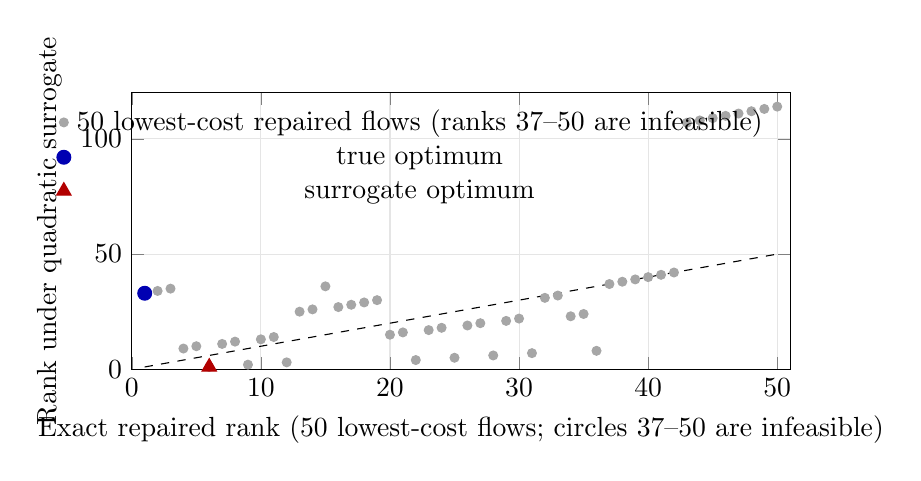
\begin{tikzpicture}
\begin{axis}[
    width=0.82\linewidth,
    height=0.42\linewidth,
    xlabel={Exact repaired rank (50 lowest-cost flows; circles 37--50 are infeasible)},
    ylabel={Rank under quadratic surrogate},
    xmin=0, xmax=51,
    ymin=0, ymax=120,
    grid=both,
    grid style={gray!20},
    legend style={draw=none, fill=none, at={(0.98,0.98)}, anchor=north east},
]
\addplot[gray!70, only marks, mark=*, mark size=1.6pt] coordinates {
(1,33) (2,34) (3,35) (4,9) (5,10) (6,1) (7,11) (8,12) (9,2) (10,13)
(11,14) (12,3) (13,25) (14,26) (15,36) (16,27) (17,28) (18,29) (19,30)
(20,15) (21,16) (22,4) (23,17) (24,18) (25,5) (26,19) (27,20) (28,6)
(29,21) (30,22) (31,7) (32,31) (33,32) (34,23) (35,24) (36,8) (37,37)
(38,38) (39,39) (40,40) (41,41) (42,42) (43,107) (44,108) (45,109)
(46,110) (47,111) (48,112) (49,113) (50,114)
};
\addlegendentry{50 lowest-cost repaired flows (ranks 37--50 are infeasible)}
\addplot[blue!70!black, only marks, mark=*, mark size=2.5pt] coordinates {(1,33)};
\addlegendentry{true optimum}
\addplot[red!70!black, only marks, mark=triangle*, mark size=3pt] coordinates {(6,1)};
\addlegendentry{surrogate optimum}
\addplot[black, dashed, domain=1:50, samples=2] {x};
\end{axis}
\end{tikzpicture}
\caption{Surrogate rank audit for the 50 lowest-cost repaired flows. Exact
enumeration confirms there are exactly 36 feasible flows (ranks 1--36); the
remaining 14 shown here are infeasible flows whose penalty values are
insufficient to place them above all feasible ones. The surrogate has high
global $R^2$ but imperfect low-energy ordering: the exact optimum is only
rank 33 under the surrogate, while the surrogate minimum repairs to the
sixth-best exact flow. Quantum-sampling outcomes are therefore scored using the
exact repaired objective $F$, not the surrogate $\widehat F$.}
\label{fig:supp-surrogate-rank}
\end{figure*}

\clearpage

\section{Exact Auxiliary Repair: Component Decomposition}
\label{sec:supp-aux-repair}

The QUBO objective $E_{\mathrm{QUBO}}(y,z)$ acts on 36 binary variables: the 19 flow (design) variables $y=(y_1,\ldots,y_{19})$ and 17 binary auxiliary (slack) variables $z=(z_1,\ldots,z_{17})$ introduced by the penalty reformulation.
A sampled 36-bit string is not directly interpretable as a flowsheet because the auxiliary bits are bookkeeping for the inequality constraints of the original design problem, not design decisions.
After projecting a sample onto the 19 flow bits $y$, the repair step finds the auxiliary assignment that minimizes the QUBO energy for that flow:
\begin{equation}
z^\star(y) = \arg\min_{z \in \{0,1\}^{17}} E_{\mathrm{QUBO}}(y, z).
\label{eq:supp-repair}
\end{equation}

Brute-force enumeration over all $2^{17} = 131{,}072$ auxiliary assignments is tractable for a single call but unnecessarily costly when repair is applied to every sampled state across all workflows.
Once $y$ is fixed, every term in $E_{\mathrm{QUBO}}$ that involves an auxiliary variable $z_k$ is either (i)~a linear term $c_k z_k$, (ii)~an auxiliary-auxiliary coupling $c_{k\ell}\,z_k z_\ell$, or (iii)~a flow-auxiliary coupling $c_{ik}\,y_i z_k$ (a constant given~$y$).
Consider the \emph{auxiliary coupling graph}: nodes are the 17 auxiliary variables, and an edge connects $z_k$ and $z_\ell$ whenever their quadratic coefficient $c_{k\ell}\neq 0$.
For this QUBO the graph has 13 connected components: 9 isolated nodes (one auxiliary bit each) and 4 edges (two auxiliary bits each).
Because there are no edges between components, fixing~$y$ makes the components conditionally independent, and \eqref{eq:supp-repair} decomposes as
\begin{equation}
\min_{z} E_{\mathrm{QUBO}}(y, z) = \mathrm{const}(y) + \sum_{c=1}^{13} \min_{z^{(c)}} E^{(c)}(y, z^{(c)}),
\end{equation}
where $z^{(c)}$ are the auxiliary bits in component~$c$ and $E^{(c)}$ contains only the terms that involve those bits (with fixed~$y$ values substituted as constants).
Each sub-problem is solved by enumerating $2^1=2$ or $2^2=4$ assignments and selecting the minimum energy; the total work is at most $9{\times}2 + 4{\times}4 = 34$ comparisons per repair, a factor of $\sim\!3{,}800\times$ smaller than the brute-force bound.
This procedure is implemented in \artifact{scripts/run\_classical\_baselines.jl}; the component structure is read from \artifact{ds\_mfg\_reduced\_flow\_objective/auxiliary\_components.csv}.

\smallskip
\noindent\textbf{Physical meaning of the components.}
Table~\ref{tab:supp-aux-components} lists all 13 components with their auxiliary variable indices, the flow variables whose fixed values enter each local energy, and a brief description.
Singleton components (1--5, 10--13) correspond to individual inequality constraints in the penalty QUBO: the single binary slack takes the value ($0$ or $1$) that satisfies the inequality, which for feasible flow assignments is the constraint residual.
Pair components (6--9) each arise from the product-linearization of the Route~B activation rule ($f_{06}=1$ iff Reactor~1 is PFR or CSTR \emph{and} Reactor~2 is Batch).
Linearizing a product of two binary variables requires up to three inequality constraints; the slack for such a constraint can take values in $\{0,1,2\}$, needing two binary bits.
The four pair components together represent the complete linearization of this one coupling rule across all Reactor~1/Reactor~2 type combinations.

\begin{table*}[t]
\centering
\footnotesize
\caption{Independent auxiliary components for the DS-MFG QUBO repair
         (source: \artifact{ds\_mfg\_reduced\_flow\_objective/auxiliary\_components.csv}).
         Variable indices 1--19 are the 19 flow variables~$y$; indices 20--36 are the 17
         binary auxiliary (slack) variables~$z$.
         \emph{Flow neighbors} are the $y$-indices that appear in the local energy $E^{(c)}$.
         No coupling term links auxiliaries across components, so each
         sub-problem is solved independently by enumeration.}
\label{tab:supp-aux-components}
\setlength{\tabcolsep}{3pt}
\begin{tabular}{L{0.04\linewidth}L{0.08\linewidth}L{0.05\linewidth}L{0.47\linewidth}L{0.05\linewidth}L{0.18\linewidth}}
\hline
\# & Aux.\ idx. & $n_{\mathrm{aux}}$ & Flow neighbors ($y$ idx.\ and $f$-arc) & $2^{n_{\mathrm{aux}}}$ & Role \\
\hline
1  & 20      & 1 & 17~($f_{16}$, Batch\,U/S),\enspace 18~($f_{17}$, cont.\ exit)
   & 2 & Batch/cont.\ downstream exclusion \\
2  & 21      & 1 & 2~($f_{01}$, PFR\,Rxn\,1),\enspace 3~($f_{02}$, CSTR\,Rxn\,1),\enspace 4~($f_{03}$, Batch\,Rxn\,1)
   & 2 & Reactor\,1 at-most-one \\
3  & 22      & 1 & 6~($f_{05}$, Route\,A),\enspace 7~($f_{06}$, Route\,B)
   & 2 & Route at-most-one \\
4  & 23      & 1 & 9~($f_{08}$, PFR\,Rxn\,2),\enspace 10~($f_{09}$, CSTR\,Rxn\,2),\enspace 11~($f_{10}$, Batch\,Rxn\,2)
   & 2 & Reactor\,2 at-most-one \\
5  & 24      & 1 & 14~($f_{13}$, Cont.\,I),\enspace 15~($f_{14}$, Cont.\,II),\enspace 16~($f_{15}$, Cont.\,III),\enspace 17~($f_{16}$, Batch\,U/S)
   & 2 & Downstream at-most-one \\
6  & 25,\,26 & 2 & 2~($f_{01}$, PFR\,Rxn\,1),\enspace 7~($f_{06}$, Route\,B),\enspace 11~($f_{10}$, Batch\,Rxn\,2)
   & 4 & Route\,B linearization (PFR\,Rxn\,1 case) \\
7  & 27,\,28 & 2 & 3~($f_{02}$, CSTR\,Rxn\,1),\enspace 7~($f_{06}$, Route\,B),\enspace 11~($f_{10}$, Batch\,Rxn\,2)
   & 4 & Route\,B linearization (CSTR\,Rxn\,1 case) \\
8  & 29,\,30 & 2 & 4~($f_{03}$, Batch\,Rxn\,1),\enspace 7~($f_{06}$, Route\,B),\enspace 11~($f_{10}$, Batch\,Rxn\,2)
   & 4 & Route\,B linearization (Batch\,Rxn\,1 case) \\
9  & 31,\,32 & 2 & 2~($f_{01}$, PFR\,Rxn\,1),\enspace 3~($f_{02}$, CSTR\,Rxn\,1),\enspace 6~($f_{05}$, Route\,A)
   & 4 & Route\,B linearization (Route\,A side) \\
10 & 33      & 1 & 6~($f_{05}$, Route\,A),\enspace 11~($f_{10}$, Batch\,Rxn\,2)
   & 2 & Route\,A\,/\,Rxn\,2 coupling \\
11 & 34      & 1 & 14~($f_{13}$, Cont.\,I),\enspace 18~($f_{17}$, cont.\ exit)
   & 2 & Cont.\,I flow balance \\
12 & 35      & 1 & 15~($f_{14}$, Cont.\,II),\enspace 18~($f_{17}$, cont.\ exit)
   & 2 & Cont.\,II flow balance \\
13 & 36      & 1 & 16~($f_{15}$, Cont.\,III),\enspace 18~($f_{17}$, cont.\ exit)
   & 2 & Cont.\,III flow balance \\
\hline
\multicolumn{6}{l}{$9{\times}2 + 4{\times}4 = 34$ comparisons per repair vs.\ $2^{17}=131{,}072$ brute force (${\sim}3{,}800{\times}$ reduction).} \\
\hline
\end{tabular}
\end{table*}

\clearpage

\section{Algorithm Parameters and Hardware Execution}
\label{sec:supp-variational}

\begin{table*}[t]
\centering
\footnotesize
\caption{Circuit parameters for the QAOA and VQE workflows reported in
         Table~1 of the main manuscript.}
\label{tab:supp-variational-provenance}
\setlength{\tabcolsep}{3pt}
\begin{tabular}{L{0.18\linewidth}L{0.16\linewidth}L{0.23\linewidth}L{0.21\linewidth}L{0.14\linewidth}}
\hline
Workflow & Circuit / ansatz & Objective and optimizer & Parameter source & Validation metric \\
\hline
Energy-targeted QAOA &
$p=5$ QAOA on the 19-flow surrogate. &
Minimize $\mathbb{E}_{p_\theta}[\widehat F(y)]$ with JuliQAOA
\texttt{find\_angles\_bh}; seed 91001; 5 basin-hopping iterations. &
\artifact{ds\_mfg\_qaoa\_juliqaoa\_angle\_search/juliqaoa\_angle\_summary.csv};
angles transferred beta-then-gamma to \texttt{QiskitOpt.QAOA}. &
664 reference hits / 262144 reads; 39661 top-50 reads. \\
\hline
Reduced-surrogate VQE &
\texttt{EfficientSU2}; 152 parameters on the 19-flow surrogate. &
COBYLA through \texttt{QiskitOpt.VQE}; 128 optimizer reads; 25 iterations;
seeds 74001, 74007, and 74018 in the final follow-up. &
Sampled distributions and optimized ansatz vectors retained in
\artifact{ds\_mfg\_vqe\_reduced\_flow\_objective\_seed74018\_metadata/} and
\artifact{ds\_mfg\_vqe\_reduced\_flow\_objective\_selected\_metadata/}. &
Seed 74018: 20 reference hits / 524288 reads; three seeds combined: 28
reference hits / 1572864 reads. \\
\hline
\end{tabular}
\end{table*}

\begin{table*}[t]
\centering
\footnotesize
\caption{Hardware pilot execution metadata retained in the submitted-job archive.}
\label{tab:supp-hardware-provenance}
\setlength{\tabcolsep}{3pt}
\begin{tabular}{L{0.24\linewidth}L{0.70\linewidth}}
\hline
Item & Metadata \\
\hline
Backend and jobs &
\texttt{ibm\_fez} (156 qubits); backend queried 2026-06-17 20:19 UTC;
9 completed jobs; 4096 shots per job; repeats 1--3; transpile seeds
92001--92003; job IDs retained in manifest. \\
\hline
Logical circuit &
19 qubits and 19 classical bits; pre-transpile depth 86; operation counts:
19~\texttt{h}, 95~\texttt{rx}, 95~\texttt{rz}, 255~\texttt{rzz}, and
19 measurements; scoring reverses Qiskit count keys to $x_1,\ldots,x_{19}$. \\
\hline
Hardware outcome &
36864 total reads; 6 top-50 reads; 4 Gurobi-pool reads;
0 reference-optimum reads; best repaired flow rank 2 ($F=11.8105$).
With zero reference hits, the two-sided 95\% Wilson upper bound on the
reference-optimum rate is $1.04\times 10^{-4}$. The pilot validates
submission and scoring; no noise mitigation was applied. \\
\hline
\end{tabular}
\end{table*}

\end{document}
